% Page: GF/EF applications against the noise-to-signal ratio of panel reviewer scores.
% GENERATED BY msca_noise_pages.py - edit that file, not this one.
% IF 2014-2018 reviewer totals (0-100); one-way ANOVA by panel; SE: bootstrap (1,000).

\clearpage
\subsection*{Noise-to-signal ratio --- 0–100 score}
\begin{center}
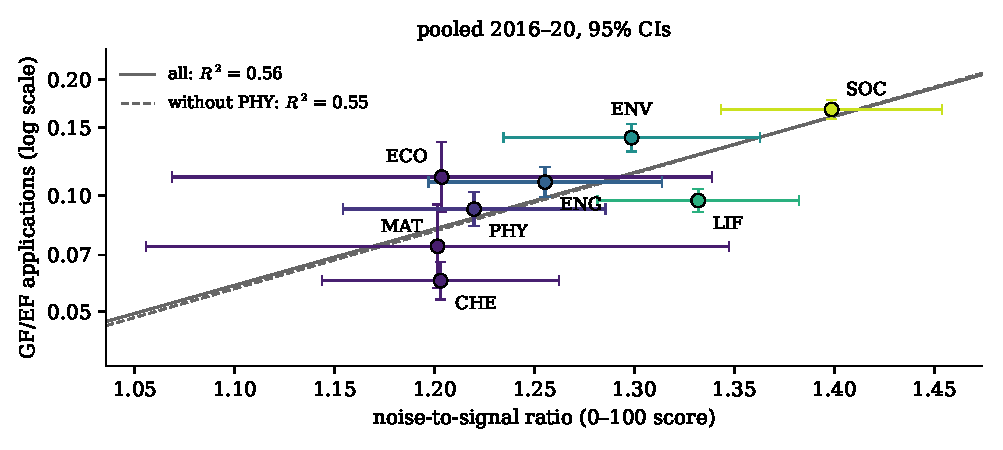
\includegraphics[width=\textwidth]{MSCA_noise_a_ns_raw.pdf}
\par\medskip
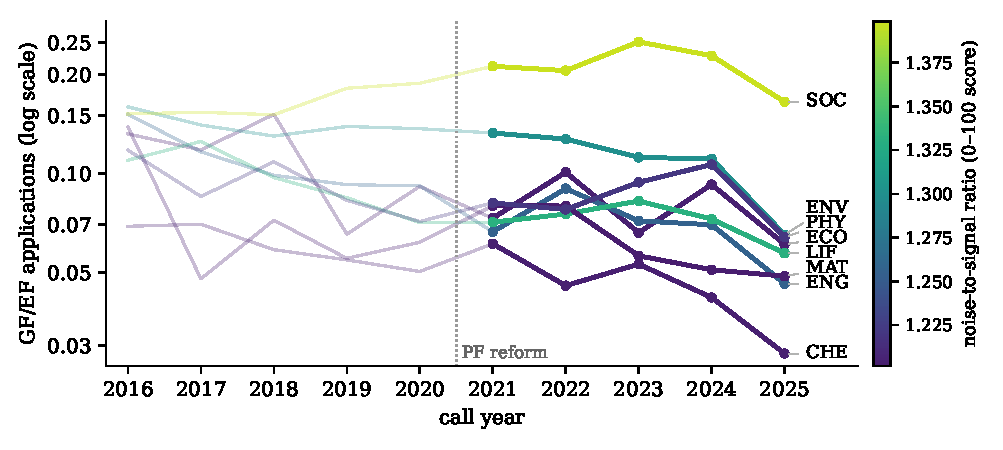
\includegraphics[width=\textwidth]{MSCA_noise_c_ns_raw.pdf}
\par\medskip
\small\renewcommand{\arraystretch}{1.15}\setlength{\tabcolsep}{4pt}
\begin{tabular}{@{}lcccccccc@{}}
\toprule
 & SOC & LIF & ENV & ENG & PHY & ECO & CHE & MAT \\
\midrule
Noise: within-proposal SD & 14.0 & 11.1 & 11.6 & 12.5 & 9.8 & 13.2 & 10.8 & 11.7 \\
Signal: between-proposal SD & 10.0 & 8.3 & 8.9 & 10.0 & 8.1 & 10.9 & 9.0 & 9.7 \\
Noise-to-signal ratio & 1.399 & 1.332 & 1.299 & 1.255 & 1.220 & 1.204 & 1.203 & 1.201 \\
SE & (0.028) & (0.026) & (0.033) & (0.030) & (0.034) & (0.069) & (0.030) & (0.074) \\
\bottomrule
\end{tabular}
\end{center}
